\documentclass[conference]{IEEEtran}
\usepackage[pdftex]{graphicx}
\usepackage{amsmath}
\usepackage{booktabs}
\usepackage{xcolor}
\usepackage{listings}
\lstset{basicstyle=\ttfamily,
	showstringspaces=false,
	commentstyle=\color{red},
	keywordstyle=\color{blue}
}
\usepackage{biblatex}
\usepackage[colorlinks=true,allcolors=black]{hyperref}
%\usepackage[backend=biber, bibencoding=utf8, style=ieee]{biblatex}
\addbibresource{references.bib}

\begin{document}
\title{Practical Assignment\\ {\fontsize{13}{0}\selectfont 2IMN15: Internet of Things } \\ {\fontsize{13}{0}\selectfont \today }\\{ \fontsize{13}{0}\selectfont Group 14: Broker Team - Blue}}

\author{\IEEEauthorblockN{Sai Krishna Kalluri}
	\IEEEauthorblockA{TU/e, Netherlands\\
		Email: saikrishh.kalluri@gmail.com}
	\and
	\IEEEauthorblockN{Snorri Stefansson}
	\IEEEauthorblockA{TU/e, Netherlands\\
		Email: snorriste@gmail.com}}
\maketitle

\IEEEpeerreviewmaketitle


\begin{abstract}
	This practical assignment for the course IoT involves creating a lightning system controlled and managed by different but relevant wireless protocols and separated individual applications. The architecture and development of this system will be the topic of this report.\\
	
\end{abstract}


\section{Introduction - Understanding the application}

Creating a lighting system with an IoT architecture may sound like an overkill, yet when the application and architecture is designed carefully it becomes essential in everyday life. This system will be described as it will be tested in the final plug fest of this course. The light system is composed of; four lights, each with a user, a user application with a UI, a sensor to detect the users presence, a manager, his web manager UI. These are the most important physical components which allow for a complete system to be operated. There are three groups which develop this system as stated in Figure \ref{fig:fig1}.

\begin{figure}[h]
	\begin{center}
		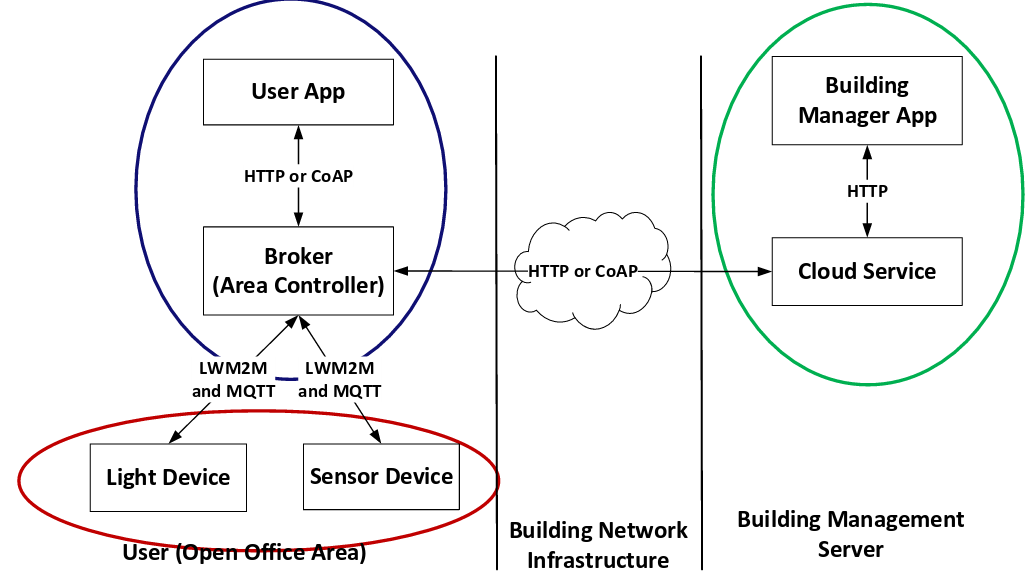
\includegraphics[width=1\linewidth]{img/design}
		\caption{This Figure is from the lecture slides on IoT \cite{slides}}
		\label{fig:fig1}
	\end{center}
\end{figure}

Each team has their purpose. This is the report of the broker, thus will be written with that perspective. Two other teams complete the total assignment, they are cloud group and end-device group and will be references as that through out the report. To shortly describe the relationship with these groups and their purpose; The cloud group is basically responsible of bookkeeping of all information important for the system and the end-device group is responsible of maintaining lights and sensors in the systems which define end device. The end device will present light upon request of the user and be able to detect a user with a camera, sensor.

There are four significant deliverables for the broker group. Each of them 
\begin{enumerate}
\item There is a user app for the user to control the light/s, which was selected to be a Android app for this showcase.
\item mDNS discovery service. Avahi was chosen for this job and is built into linux or can be used with python for integration into a python project.
\item LWM2M (Rest API) - a 'light weight machine to machine communication' with end device as well as maintaining a CoAP/HTTP server. Leshan was chosen for this task and is written in Java.
\item MQTT broker which allows lights and sensors to communicate basic commands between one and other. Mosquitto was used for this and installed on linux.
\end{enumerate}

\textit{A laptop with Ubuntu 16.04 64-bit was used to run all these modules except the Android app which was run with a emulator and designed on a Windows computer.}




\section{Architecture and Protocols}

The architecture is somewhat predefined but many design options were left up to the teams. All communication and information will pass through the broker on its way to the endpoint. 

\begin{figure}[h]
	\begin{center}
		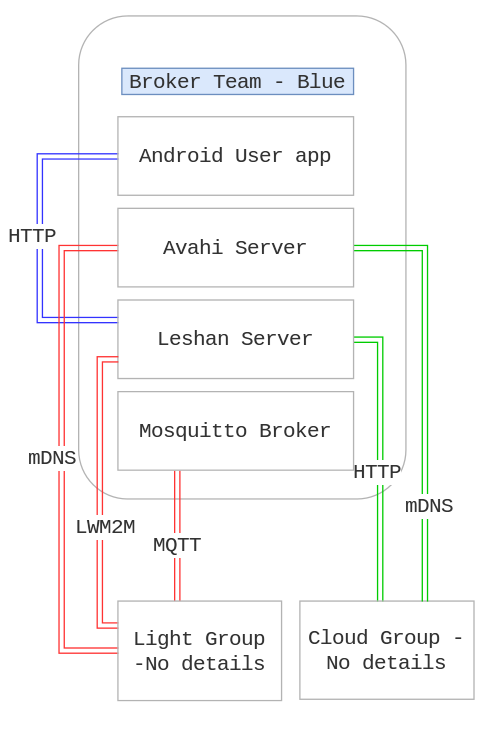
\includegraphics[width=1\linewidth]{img/overview}
		\caption{}
		\label{fig:fig2}
	\end{center}
\end{figure}
\subsection{LWM2M, CoAP and HTTP with Leshan}
Leshan infrastructure, protocols used and relevance to project

\subsection{mDNS with Avahi server}
\subsection{MQTT with Mosquitto}
\subsection{User app - Android}

\begin{figure}[h]
	\begin{center}
		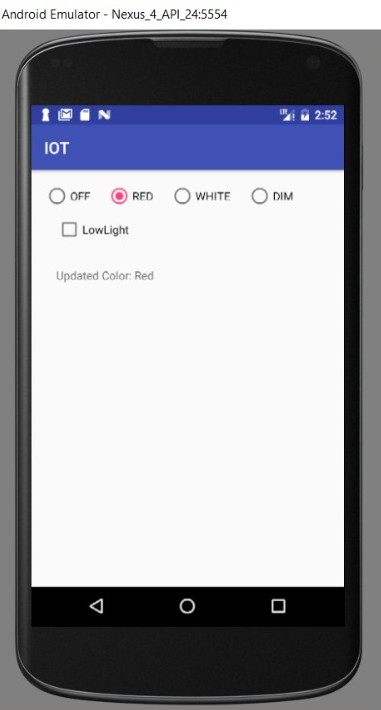
\includegraphics[width=1\linewidth]{img/androidapp}
		\caption{}
		\label{fig:fig3}
	\end{center}
\end{figure}


\section{Operations}

\subsection{Initialization}

\subsection{Use cases - post init}

\subsection{Product Testing}

\section{Discussion and results}

\section{Conclusion}






\begin{lstlisting}[basicstyle=\tiny,language=python,caption={Code}]

Code snippet
\end{lstlisting}

\printbibliography

\end{document}